\newpage
\subsection{Arquitecura del modelo de clasificación y análisis cromático}

Este modelo aborda el proceso de entrada y salida para la identificación de patrones tanto de forma local como apoyado de AWS.

\begin{figure}[H]
    \centering
    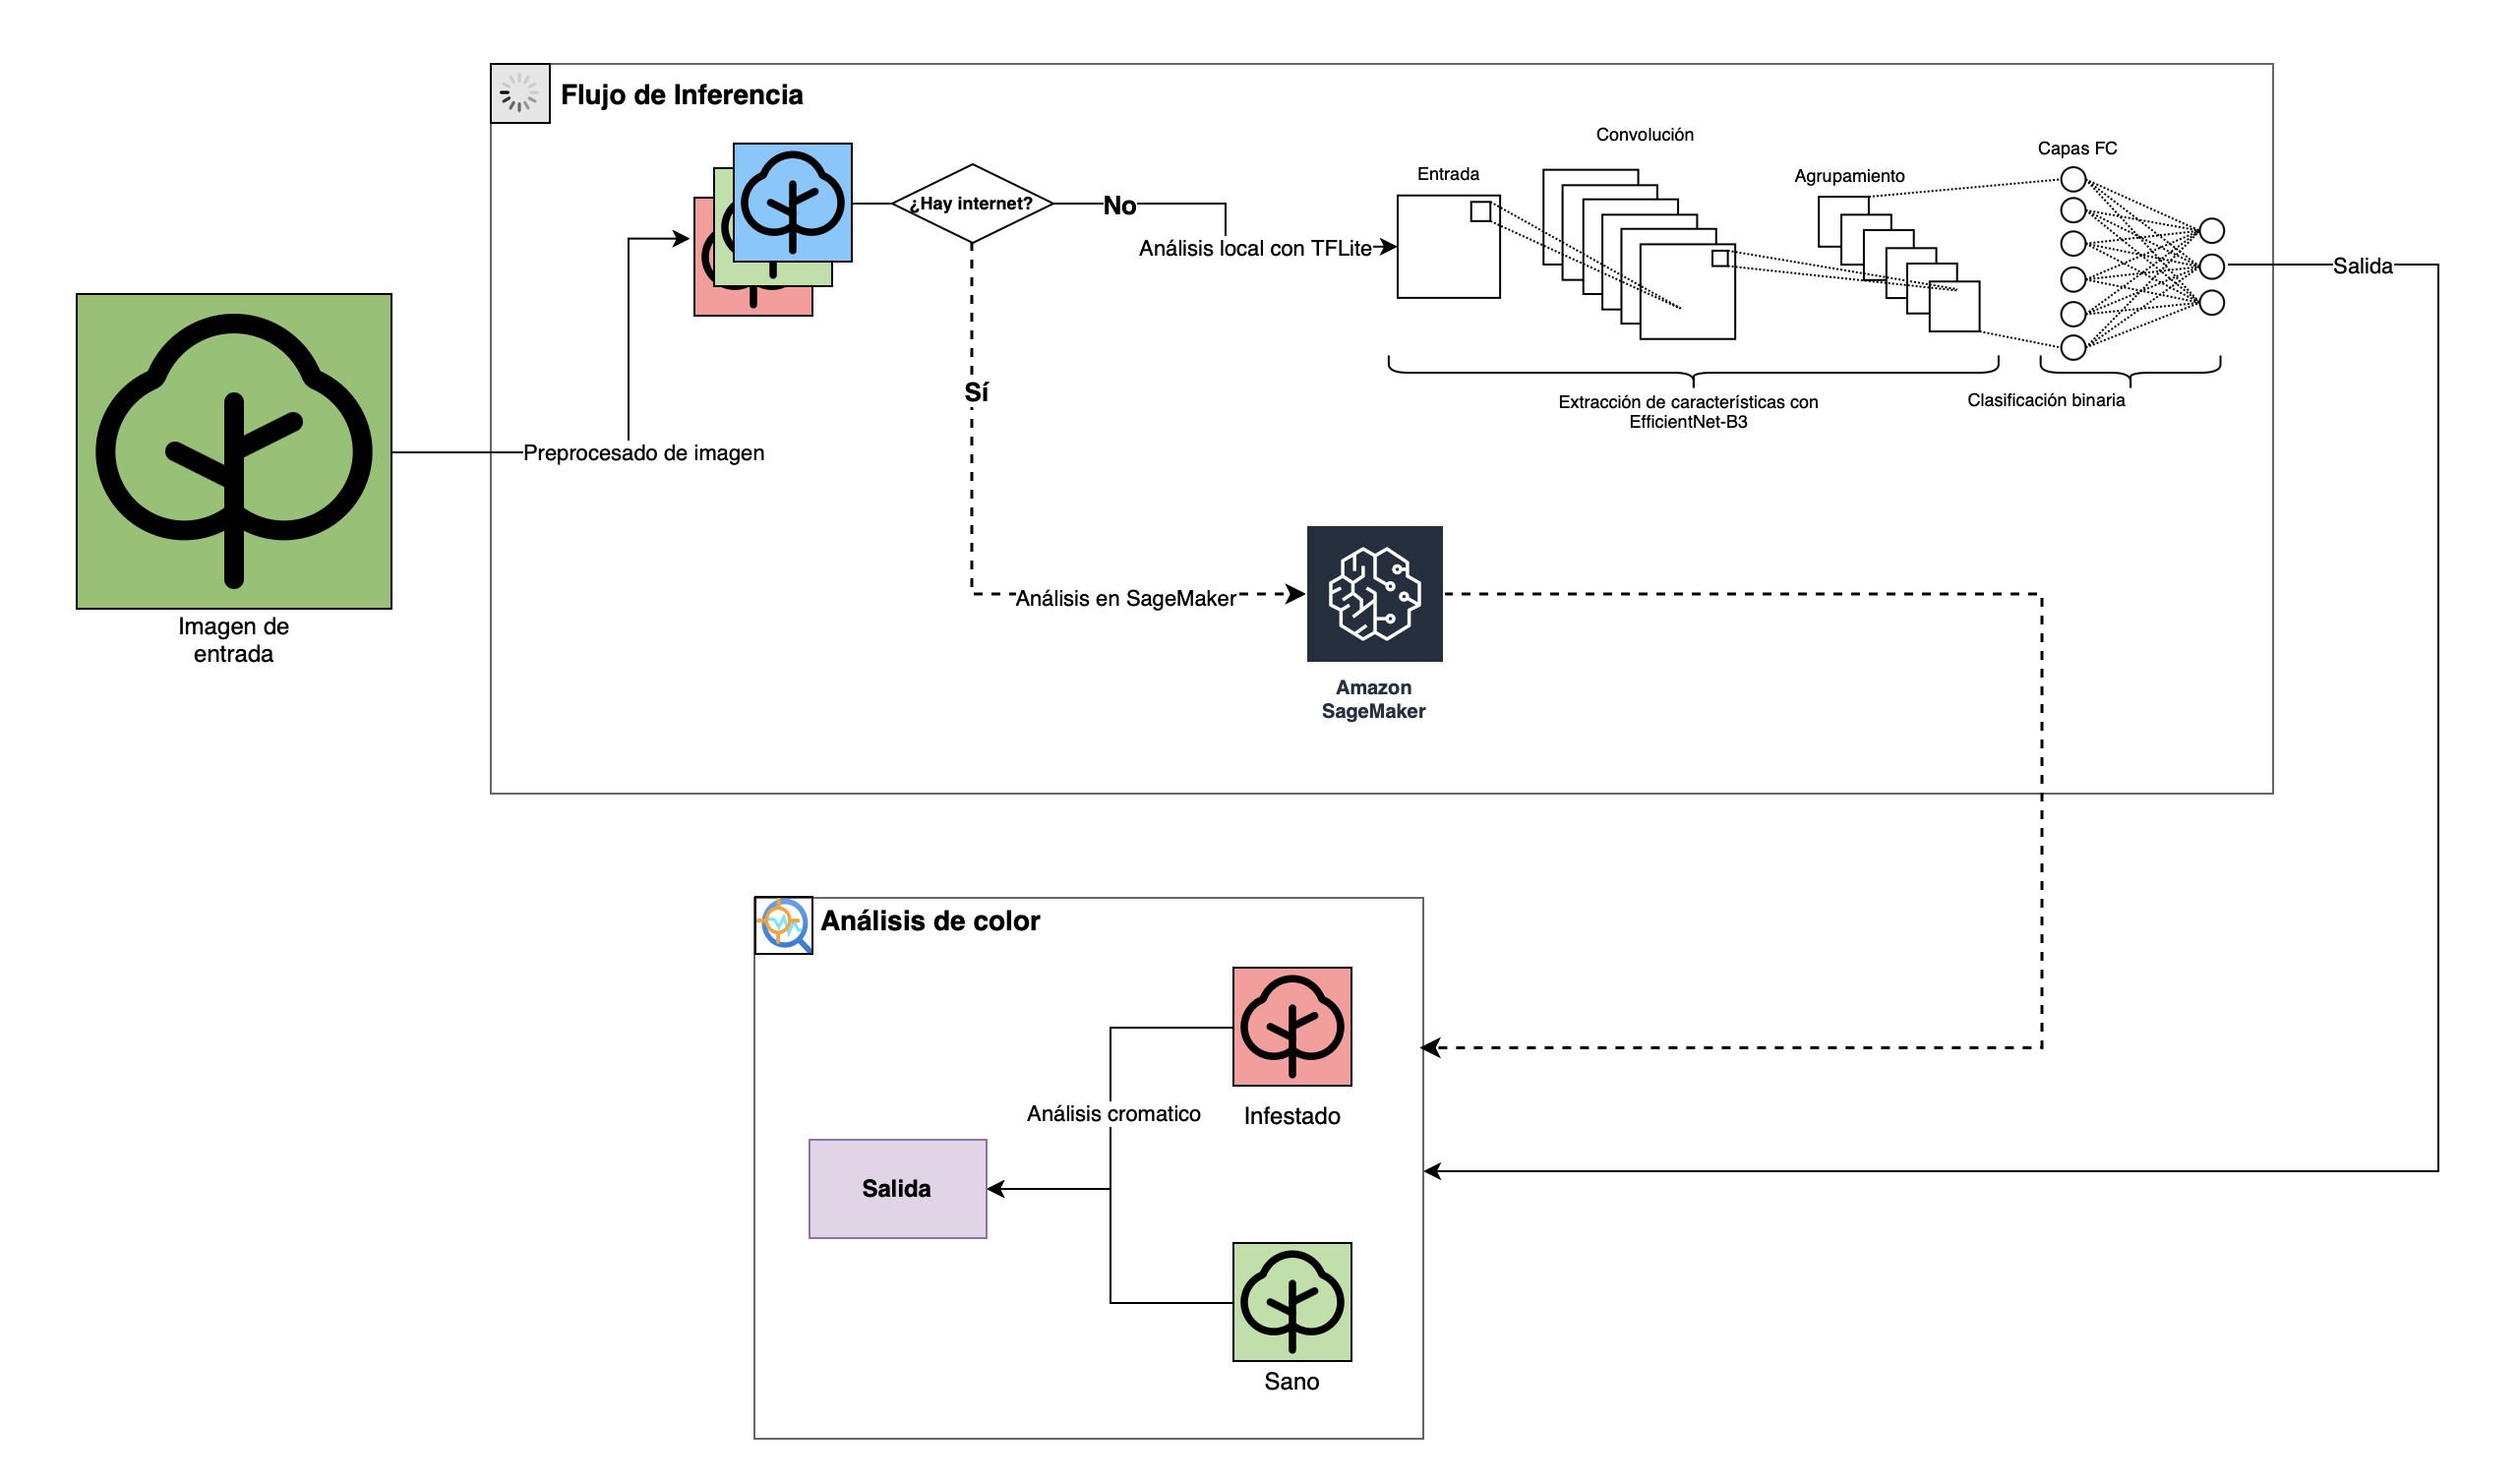
\includegraphics[width=1\textwidth]{images/C8/arq_modelo.png}
    \caption{Arquitectura general del modelo}
    \label{fig:arq_modelo}
\end{figure}

La Figura~\ref{fig:arq_modelo} ilustra el flujo completo de inferencia del sistema, desde la captura de la imagen hasta la generación del resultado final. El proceso se divide en dos etapas principales: el flujo de inferencia mediante el modelo de clasificación y el análisis cromático complementario.

En la primera etapa, la imagen de entrada —correspondiente a una fotografía de la corteza de un árbol capturada desde la aplicación móvil— es sometida a un preprocesado que la adecúa al formato requerido por el modelo: redimensionamiento a $300 \times 300$ píxeles y normalización mediante \texttt{efficientnet.preprocess\_input}. Una vez preprocesada,
el sistema evalúa el acceso a internet para determinar la ruta de inferencia. Si no hay conexión, el análisis se ejecuta localmente en el dispositivo mediante el modelo local con TFLite embebido en la aplicación móvil, garantizando la operación en zonas del Bosque de Chapultepec con cobertura de red limitada. Si hay conexión disponible, la imagen es enviada a Amazon SageMaker para su procesamiento en la nube, lo que permite aprovechar mayor capacidad de cómputo y facilitar el reentrenamiento del modelo con nuevas muestras capturadas. En ambos casos, la imagen atraviesa la arquitectura EfficientNet-B3, que extrae características visuales mediante capas de convolución y agrupamiento, y las transfiere a las capas densas que ejecutan la clasificación binaria, produciendo una salida con la probabilidad de infestación.

En la segunda etapa, el resultado de la clasificación  independientemente de si provino del dispositivo o de SageMaker— es enviado al módulo de análisis de color. Este módulo aplica un análisis cromático sobre la imagen original para complementar la predicción:
si el árbol es clasificado como infestado, se analiza la distribución de tonalidades en la corteza en busca de patrones asociados a daño por descortezadores, como cambios en la pigmentación derivados de la pérdida de resina.
El resultado combinado de ambos análisis es consolidado en la salida final del sistema, que reporta el estado del árbol (sano o infestado).
